\documentclass[a4paper,12pt]{report} % добавить leqno в [] для нумерации слева

%%% Работа с русским языком
\usepackage{cmap}					% поиск в PDF
\usepackage{mathtext} 				% русские буквы в формулах
\usepackage[T2A]{fontenc}			% кодировка
\usepackage[utf8]{inputenc}			% кодировка исходного текста
\usepackage[english,russian]{babel}	% локализация и переносы

%%% Дополнительная работа с математикой
\usepackage{amsmath,amsfonts,amssymb,amsthm,mathtools} % AMS
\usepackage{icomma} % "Умная" запятая: $0,2$ --- число, $0, 2$ --- перечисление

%% Номера формул
\mathtoolsset{showonlyrefs=true} % Показывать номера только у тех формул, на которые есть \eqref{} в тексте.

%% Шрифты
\usepackage{euscript}	 % Шрифт Евклид
\usepackage{mathrsfs} % Красивый матшрифт

%% Свои команды
\DeclareMathOperator{\sgn}{\mathop{sgn}}

%\setlength\parindent{0ex}
%\setlength\parskip{0.3cm}

%%% Заголовок
\author{Волков Павел А-14-19}
\title{Типовой расчет №17 по численным методам Вариант 3}
\date{\today}

\usepackage{graphicx}

\begin{document} % конец преамбулы, начало документа

\maketitle

\newpage
\section*{Задание}

Функция $y = y(x)$, задана таблицей своих значений.

\[
\begin{array}{| c | c | c | c | c |}
	\hline
	x & 0 & 1 & 2 & 3  \\ \hline
	y & 0 & 6 & 20 & 41  \\ \hline
\end{array}
\]

Построить параболический сплайн дефекта 1 для функции $y = y(x)$, если известно также дополнительное условие $S''(1 - 0) = S''(1 + 0)$. На одном чертеже построить график сплайна и указать исходные точки.

УКАЗАНИЕ: Для упрощения вычислений  записать многочлен на отрезке $[x_{i-1}, x_i]$ в виде $P_i(x) = a_{i, 0} + a_{i, 1}(x - x_{i-1}) + a_{i, 2}(x - x_{i-1})(x - x_i)$

\section*{Решение}

Запишем все условия на сплайн:

\begin{gather}
	P_0(0) = 0 = a_{0, 0}\\
	P_0(1) = 6 = a_{0, 1}\\
	P_1(1) = 6 = a_{1, 0}\\
	P_1(2) = 20 = 6 + a_{1, 1}\\
	P_2(2) = 20 = a_{2, 0}\\
	P_2(3) = 41 = 20 + a_{2, 1}\\
	P_0'(1) = P_1'(1) \\
	P_1'(2) = P_2'(2) \\
	P_0''(1) = P_1''(1) = a_{0, 2} = a_{1, 2}
\end{gather}

Из условий непрерывности производной сплайна получаем следующую систему:


\[
	\left\{
		\begin{aligned}
		a_{0, 2} + a_{1, 2} = 8\\
		a_{1, 2} + a_{2, 2} = 7 \\
		a_{0, 2} = a_{1, 2}
		\end{aligned}
	\right.
\]

Решив которую получаем: $a_{0, 2} = a_{1, 2} = 4$ и $a_{2, 2} = 3$

\[
	S_2(x) = 
	\left\{
		\begin{aligned}
		P_{2, 0}(x) = 6x + 4x(x - 1), x \in [0, 1]\\
		P_{2, 1}(x) = 6 + 14(x - 1) + 4(x - 1)(x - 2), x \in [1, 2] \\
		P_{2, 2}(x) = 20 + 21(x - 2) + 3(x - 2)(x - 3), x \in [2, 3]
		\end{aligned}
	\right.
\]

График сплайна:

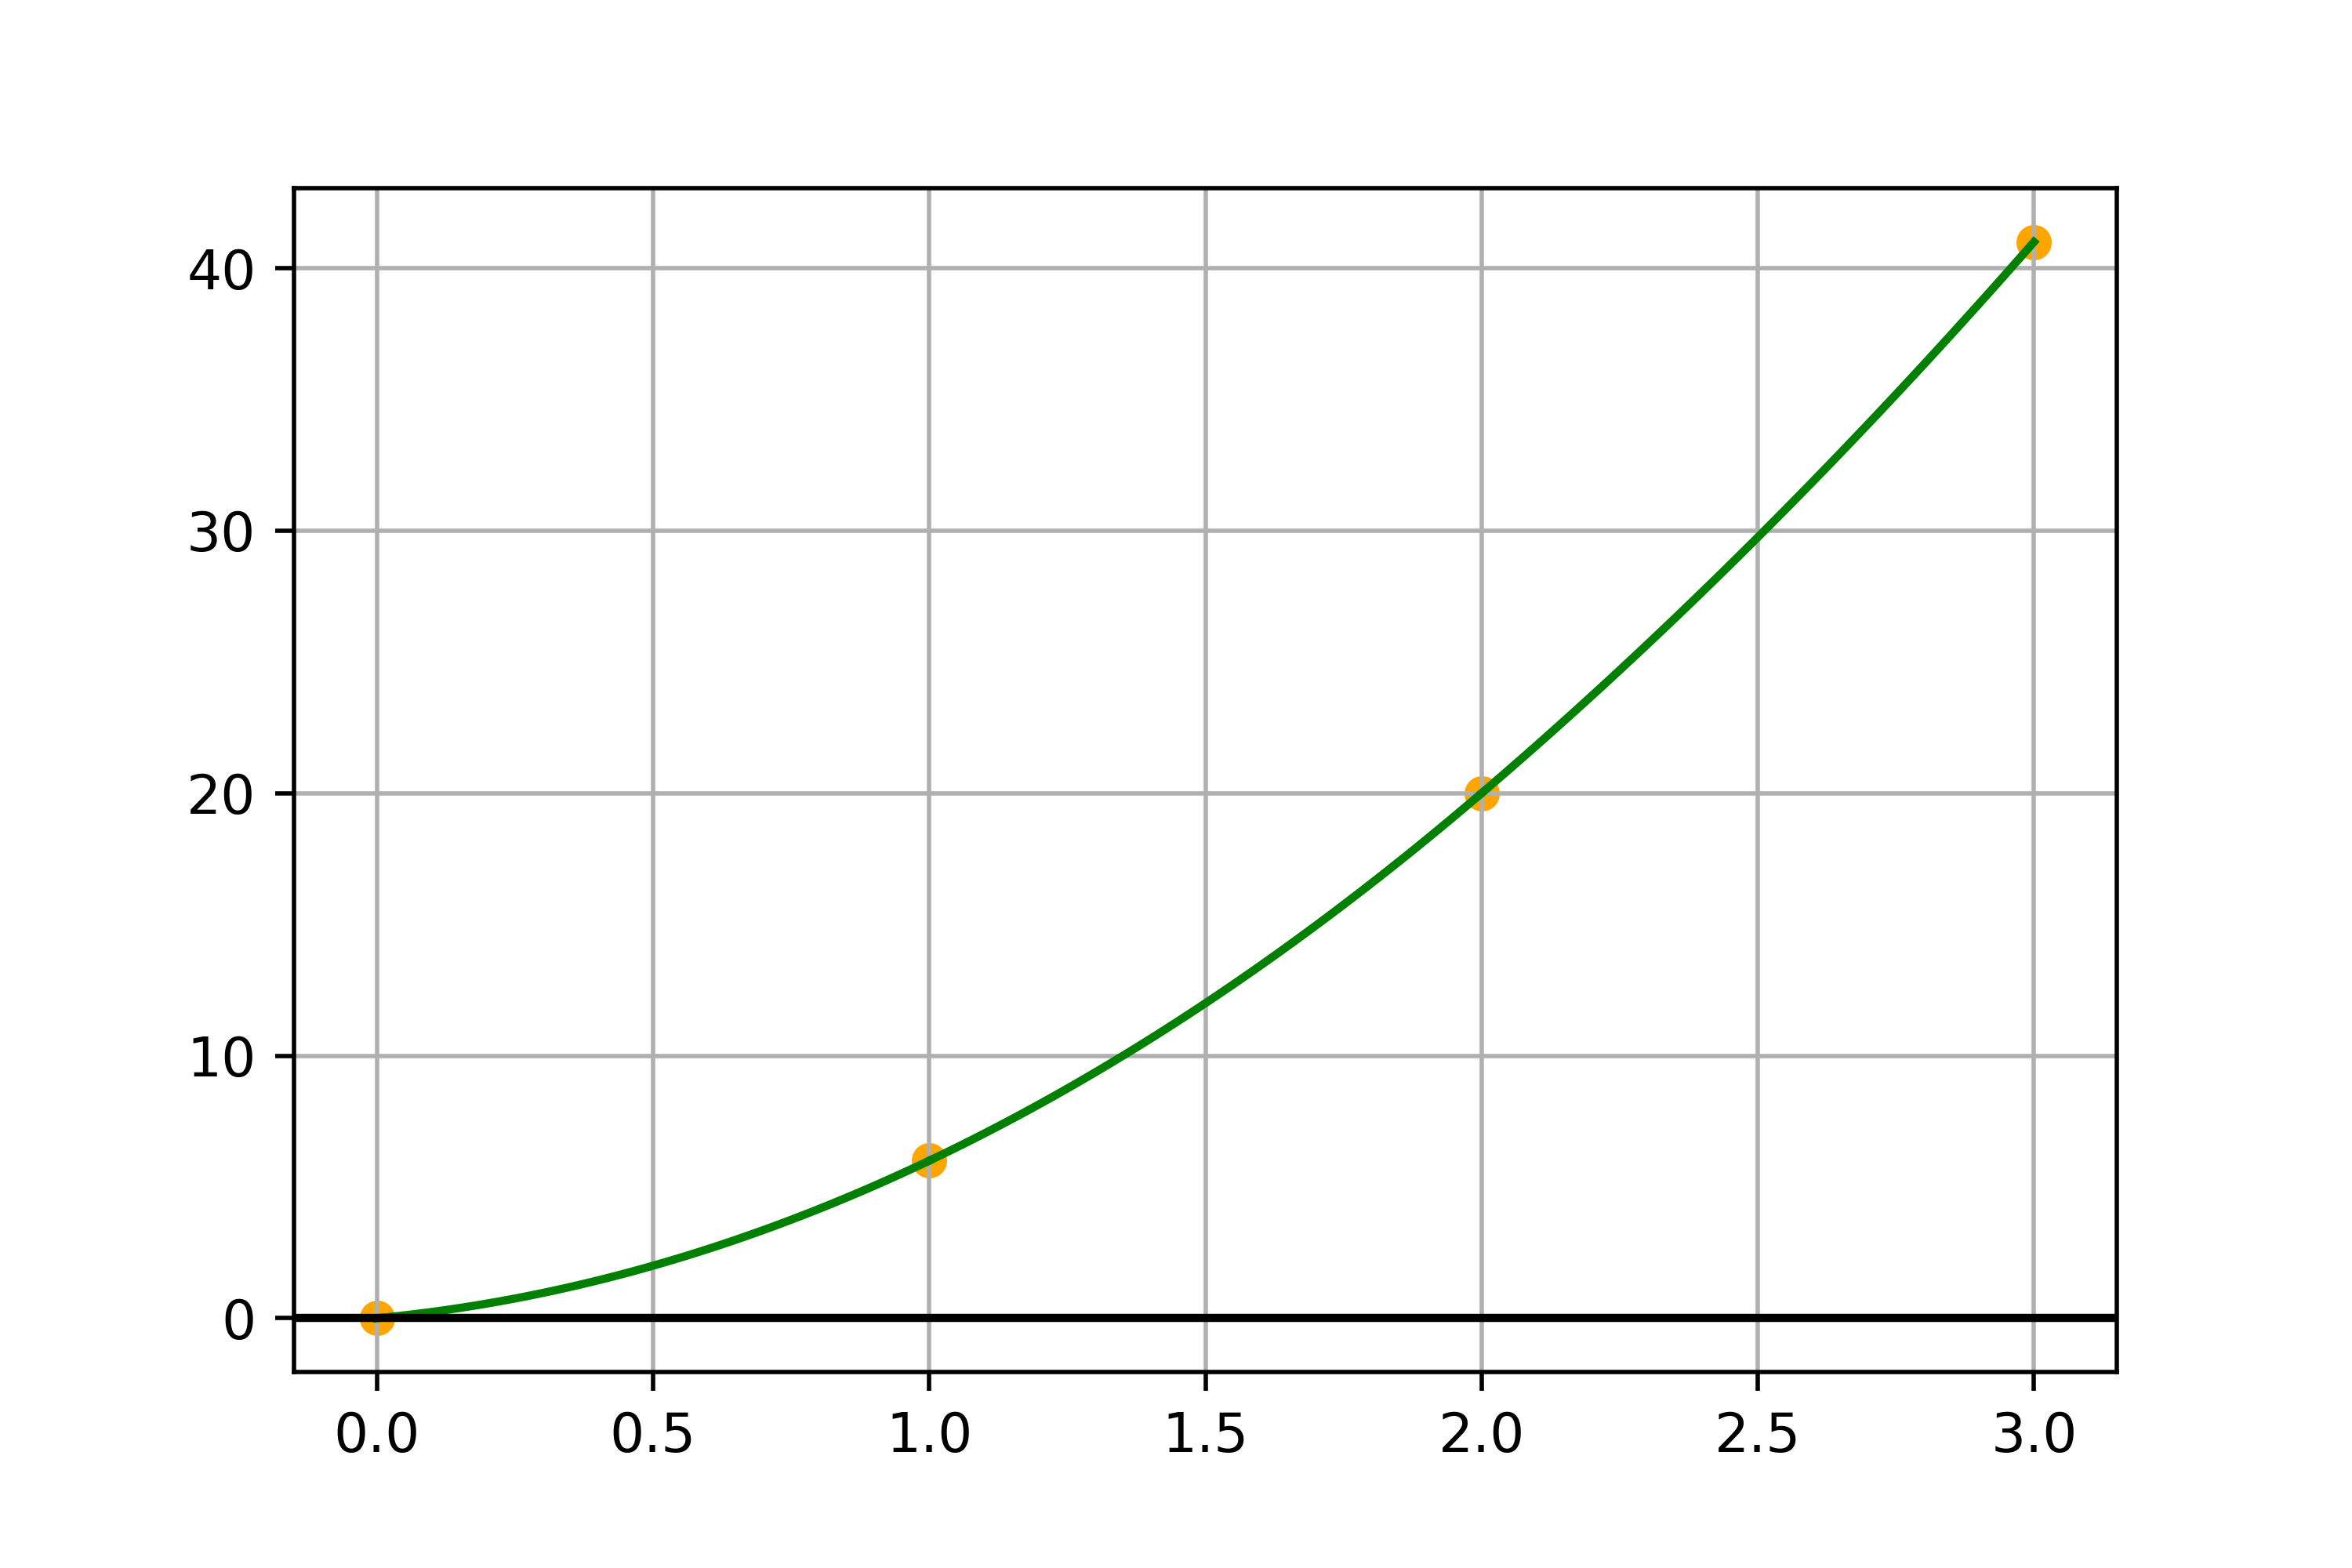
\includegraphics{regular_calc_17.png}
\end{document}